\documentclass[border=5pt]{standalone}
\usepackage{tikz}
\usepackage{bm}
\usetikzlibrary{decorations.markings,decorations.pathreplacing,calc,arrows.meta}

\tikzset{help lines/.style={very thin,color=gray!50}} % modify the help lines style
\tikzset{->-/.style={decoration={
  markings,
  mark=at position .5 with {\arrow{>}}},postaction={decorate}}}

\newcommand{\vecbf}[1]{\bm{#1}}

\begin{document}
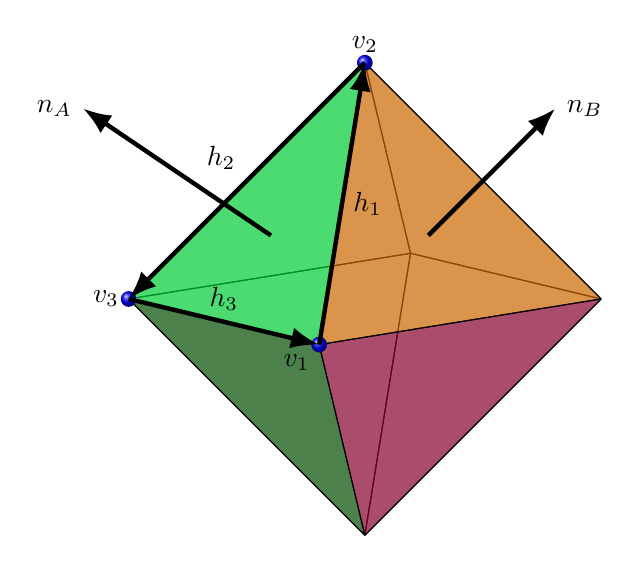
\begin{tikzpicture}[line join=bevel,z=-5.5]
	% \draw[help lines] (-10,-10) grid (10,10); %grid
    \coordinate (A1) at (0,0,-3);
    \coordinate (A2) at (-3,0,0);
    \coordinate (A3) at (0,0,3);
    \coordinate (A4) at (3,0,0);
    \coordinate (B1) at (0,3,0);
    \coordinate (C1) at (0,-3,0);
    
    \coordinate (Acenter) at (-1, 1, 1);
    \coordinate (Bcenter) at (1, 1, 1);

    \draw (A1) -- (A2) -- (B1) -- cycle;
    \draw (A4) -- (A1) -- (B1) -- cycle;
    \draw (A1) -- (A2) -- (C1) -- cycle;
    \draw (A4) -- (A1) -- (C1) -- cycle;
    \draw [fill opacity=0.7,fill=green!80!blue] (A2) -- (A3) -- (B1) -- cycle;
    \draw [fill opacity=0.7,fill=orange!80!black] (A3) -- (A4) -- (B1) -- cycle;
    \draw [fill opacity=0.7,fill=green!30!black] (A2) -- (A3) -- (C1) -- cycle;
    \draw [fill opacity=0.7,fill=purple!70!black] (A3) -- (A4) -- (C1) -- cycle;

    \shade[ball color=blue] (A3) circle (0.1) node [below left] {$v_1$};
    \shade[ball color=blue] (B1) circle (0.1) node [above] {$v_2$};
    \shade[ball color=blue] (A2) circle (0.1) node [left] {$v_3$};

    \draw[ultra thick, -Latex] (A3) --node[right] {$h_1$}  (B1);
    \draw[ultra thick, -Latex] (B1) --node[above left] {$h_2$}  (A2);
    \draw[ultra thick, -Latex] (A2) --node[above ] {$h_3$}  (A3);
    \draw[ultra thick, -Latex] (Acenter) -- ++(-2, 2, 2) node[left] {$n_A$};
    \draw[ultra thick, -Latex] (Bcenter) -- ++(2, 2, 2) node[right] {$n_B$};
    

\end{tikzpicture}

\end{document}
